\chapter{Fachklassenmodell}\label{ch:fachklassenmodell}


\section{Beziehungsdiagramm}\label{sec:beziehungsdiagramm}


\section{Fachklassendiagramm}\label{sec:fachklassendiagramm}
\begin{figure}[H]
    \centering
    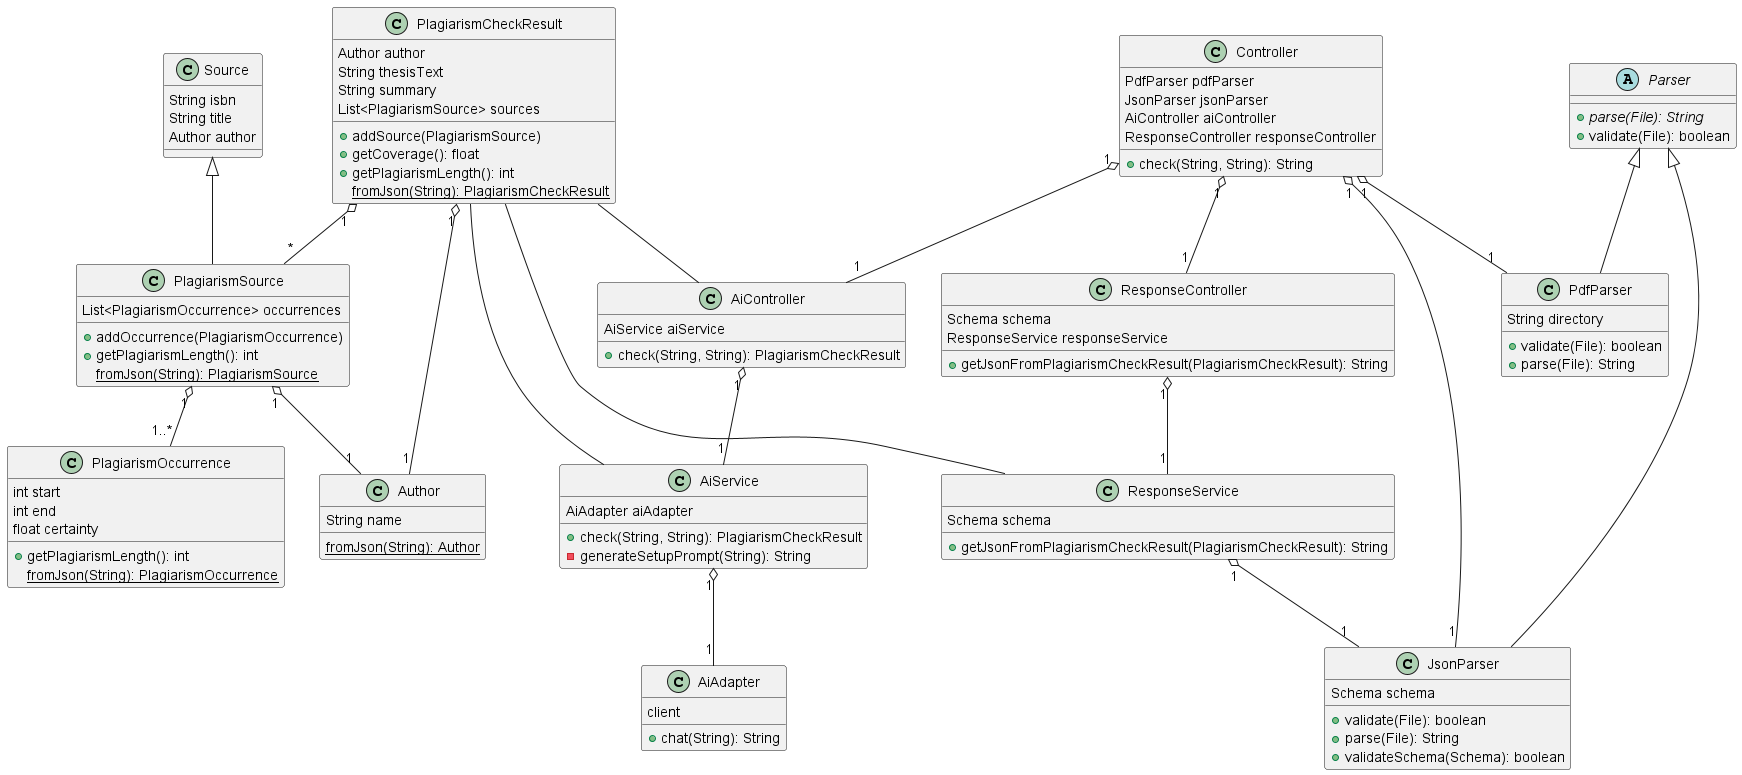
\includegraphics[width=\textwidth]{images/diagrams/Klassendiagramm}
    \caption{Fachklassendiagramm}
    \label{fig:fachklassendiagrammw}
\end{figure}


\section{Beschreibung der Fachklassen}\label{sec:beschreibung_der_fachklassen}

\subsection{Controller}\label{subsec:controller}
Dies ist die Hauptsteuerungsklasse,
sie ist verantwortlich für die Abwicklung der Anfragen und Antworten in der Anwendung.

\subsection{Author}\label{subsec:author}
Das Author Modell stellt einen Autor dar und enthält recht einfach den Namen des Autors als Feld.

\subsection{Source}\label{subsec:source}

\subsection{PlagiarismCheck}\label{subsec:plagiarism_check}

\subsection{PlagiarismCheckResult}\label{subsec:plagiarism_check_result}

\subsection{PlagiarismSource}\label{subsec:plagiarism_source}

\subsection{PlagiarismOccurrence}\label{subsec:plagiarism_occurrence}
Dieses Modell repräsentiert eine einzelne Quelle eines möglichen Plagiats.
Es enthält Informationen über die ISBN, den Titel,
den Autor der Quelle, und die Stellen, an denen das Plagiat aufgetreten ist.

\subsection{AI}\label{subsec:ai}

\subsubsection{AiController}\label{subsubsec:ai_controller}

\subsubsection{AiService}\label{subsubsec:ai_service}
Die AiService Klasse stellt einen Dienst zur Überprüfung von potenziellen Plagiaten in einem Text unter Verwendung eines KI-Adapters bereit.

\subsubsection{AiAdapter}\label{subsubsec:ai_adapter}
Die AiAdapter-Klasse ist für die Kommunikation mit der AI-Engine verantwortlich, die die Plagiatsprüfung durchführt.
Die Klasse nimmt Texteingaben von Benutzern entgegen und sendet sie an die AI-Engine zur Analyse.
Diese sendet dann eine Antwort zurück, die von der AiAdapter -Klasse weiterverarbeitet wird.

\subsection{Response}\label{subsec:response}

\subsubsection{ResponseController}\label{subsubsec:response_controller}

\subsubsection{ResponseService}\label{subsubsec:response_service}

\subsection{Utils}\label{subsec:utils}

\subsubsection{Parser}\label{subsubsec:parser}

\subsubsection{PdfParser}\label{subsubsec:pdf_parser}

\subsubsection{JsonParser}\label{subsubsec:json_parser}`